%\documentclass[12pt]{report}
%\usepackage{graphicx}
%\setlength{\parindent}{0mm}
%\setlength{\parskip}{14pt}
%\renewcommand{\baselinestretch}{2.0}
%\setlength{\topmargin}{0pt}
%\setlength{\headheight}{0pt}
%\setlength{\headsep}{0pt}
%\setlength{\footskip}{45pt}
%\setlength{\textwidth}{465pt}
%\setlength{\textheight}{660pt}
%\setlength{\oddsidemargin}{10pt}
%\newcommand{\RR}{\mathrm{I\!R\!}}
%\newcommand{\FF}{\mathrm{I\!F\!}}
%\newcommand{\dt}{\frac{\partial}{\partial t}}
%\newcommand{\dq}{\frac{\partial}{\partial q }}
%\newcommand{\dr}{\frac{\partial}{\partial p }}
%\newtheorem{defi}{Definition}[chapter]
%\newtheorem{theo}{Theorem}[chapter]


%\begin{document}

\chapter{Examination of Classical Flows}

\section{Flow Over a Flat Plate}

Using a similarity transform, we look for a stream function $\psi(x,y)$ in the form 
$$\psi(x,y) = \sqrt{(\nu U_0 x)}f(\eta)\ \ \ \ \ \eta = y \sqrt{\frac{U_0}{\eta x}}.$$

After simplification, we arrive at $$f'''(\eta) + \frac{1}{2}f(\eta)f''(\eta) = 0$$
which is Blasius equation. It is subject to the boundary conditions 
$$ y=0: V_x = 0 \ \ \  \eta = 0, f'(0) = 0$$
$$ y=0: V_y = 0 \ \ \  \eta = 0, f(0) = 0$$
$$ y=\infty: V_x = U_0 \ \ \  \eta = 0, f'(\infty) = 1.$$
The friction on the lower plate is proportional to $f''(0) \approx 0.332$. In order to confirm this result using Nast2d, we simulated a flow over a flat plate as follows.  
We solve the 2-D Navier-Stokes equation until we reach steady state. We used the following physical parameters. The length of the plate was chosen to be $30$ and the inflow velocity is $U_0 = 1$. The Reynolds number for the flow was taken to be $500,000$. A plate moving with a velocity equal to the inflow velocity was placed above the flow region. We found that there is a small region close to the lower boundary in which the effect of viscosity is pronounced. Far from the lower boundary, the flow is almost uniform. We have provided the velocity profile in Figure (\ref{blasiusvp}) and we have given few numerical values from our computation in Table(\ref{table1}). Steady state was reached at approximately $t = 2000$. We obtained the approximate value $f''(0) \approx .2645$ by using the similarity profile for $x = 15$. This similarity profile is given in Figure(\ref{blasius5}). There is a relative error of approximatly $20\%$ with the theoretical value. Such error may be attributed to several causes including the fact that steady state was reached approximatly in our computations or from rounding errors.  

\begin{figure}
\label{blasiusvp}
\begin{center}
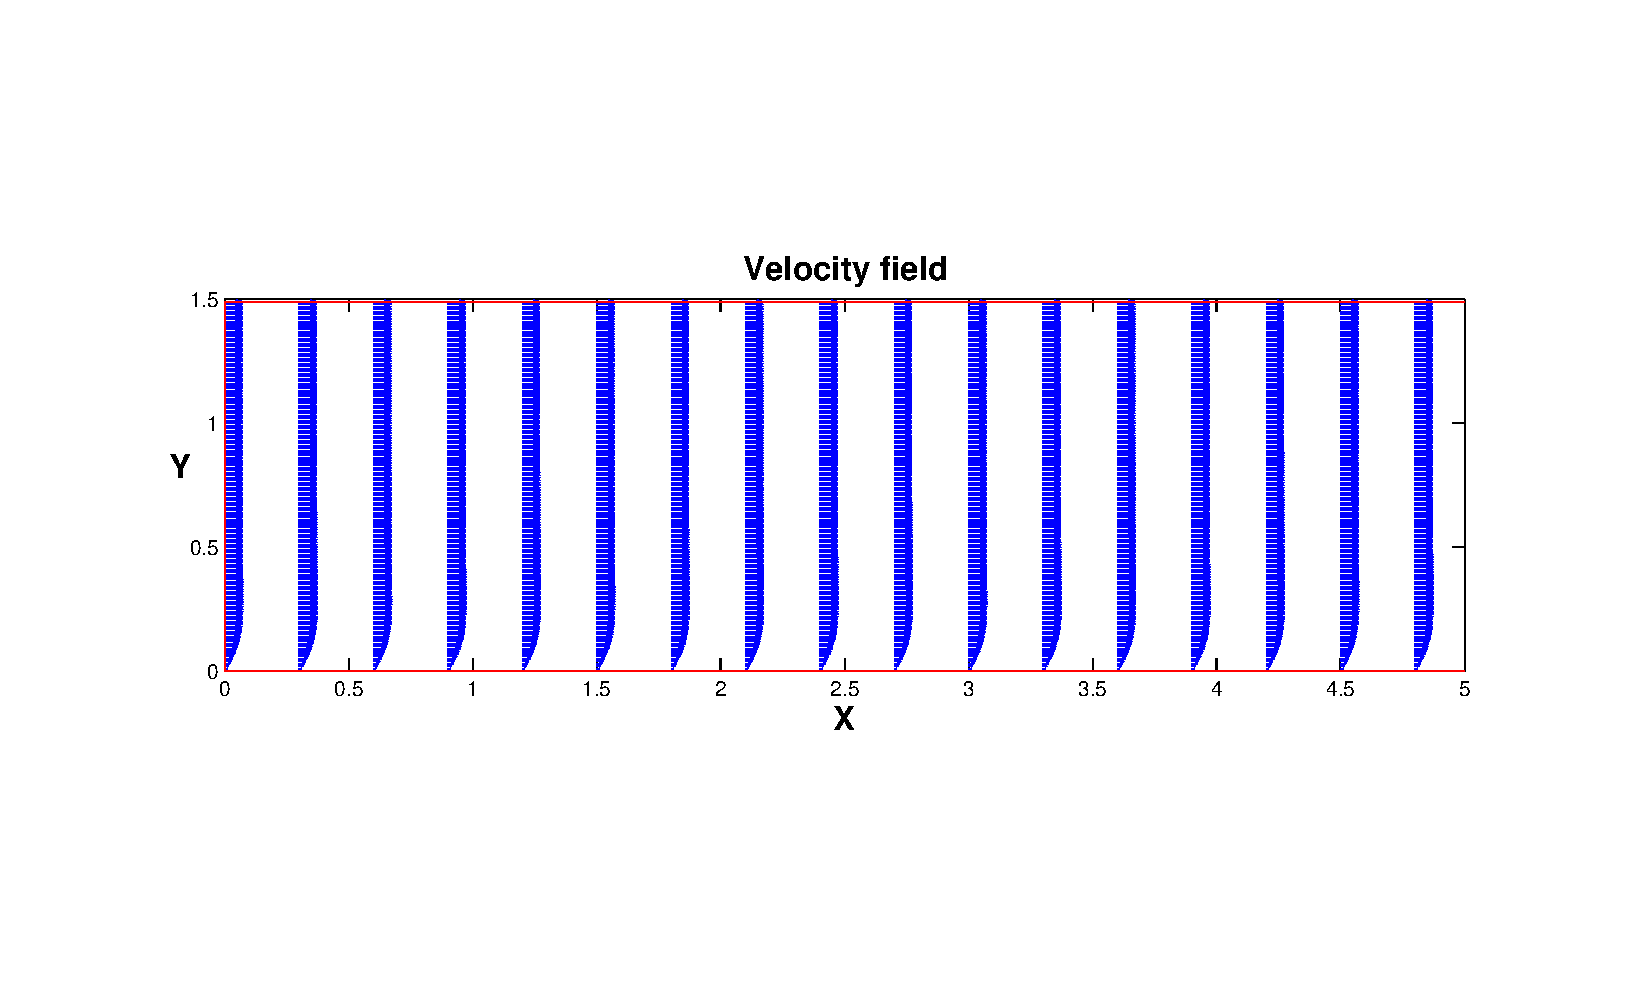
\includegraphics[scale=.4]{blasiusvp.eps}
\end{center}
\caption{Flow Between Two Parallel Plates at $Re = 500,000$}
\end{figure}

\begin{figure}
\label{blasius5}
\begin{center}
\includegraphics[scale=.4]{blasius.eps}
\end{center}
\caption{Flow Between Two Parallel Plates at $Re = 500,000$}
\end{figure}

\begin{table}
\label{table1}
\caption{Velocity in the $x$-direction vs. similarity variable at $x = 15$}
\begin{center}
\begin{tabular}{c|c}
\hline
$V_x/U_0$  &  $\eta$\\
\hline
0.044572&	0\\
0.13274	& 0.333333333\\
0.218923&	0.666666667\\
0.302261&	1\\
0.382128&	1.333333333\\
0.458035&	1.666666667\\
0.529589&	2\\
0.596505&	2.333333333\\
0.658584&	2.666666667\\
0.715718&	3\\
0.767876&	3.333333333\\
0.815102&	3.666666667\\
0.857504&	4\\
0.895244&	4.333333333\\
0.928534&	4.666666667\\
0.957621&	5\\
0.98278	& 5.333333333\\
1.004308&	5.666666667\\
1.022511&	6\\
1.037705&	6.333333333\\
1.0502	& 6.666666667\\
\hline
\end{tabular}
\end{center}
\end{table}


\section{Flow Between Two Parallel Plates}

\begin{figure}
\label{fbtpp500}
\begin{center}
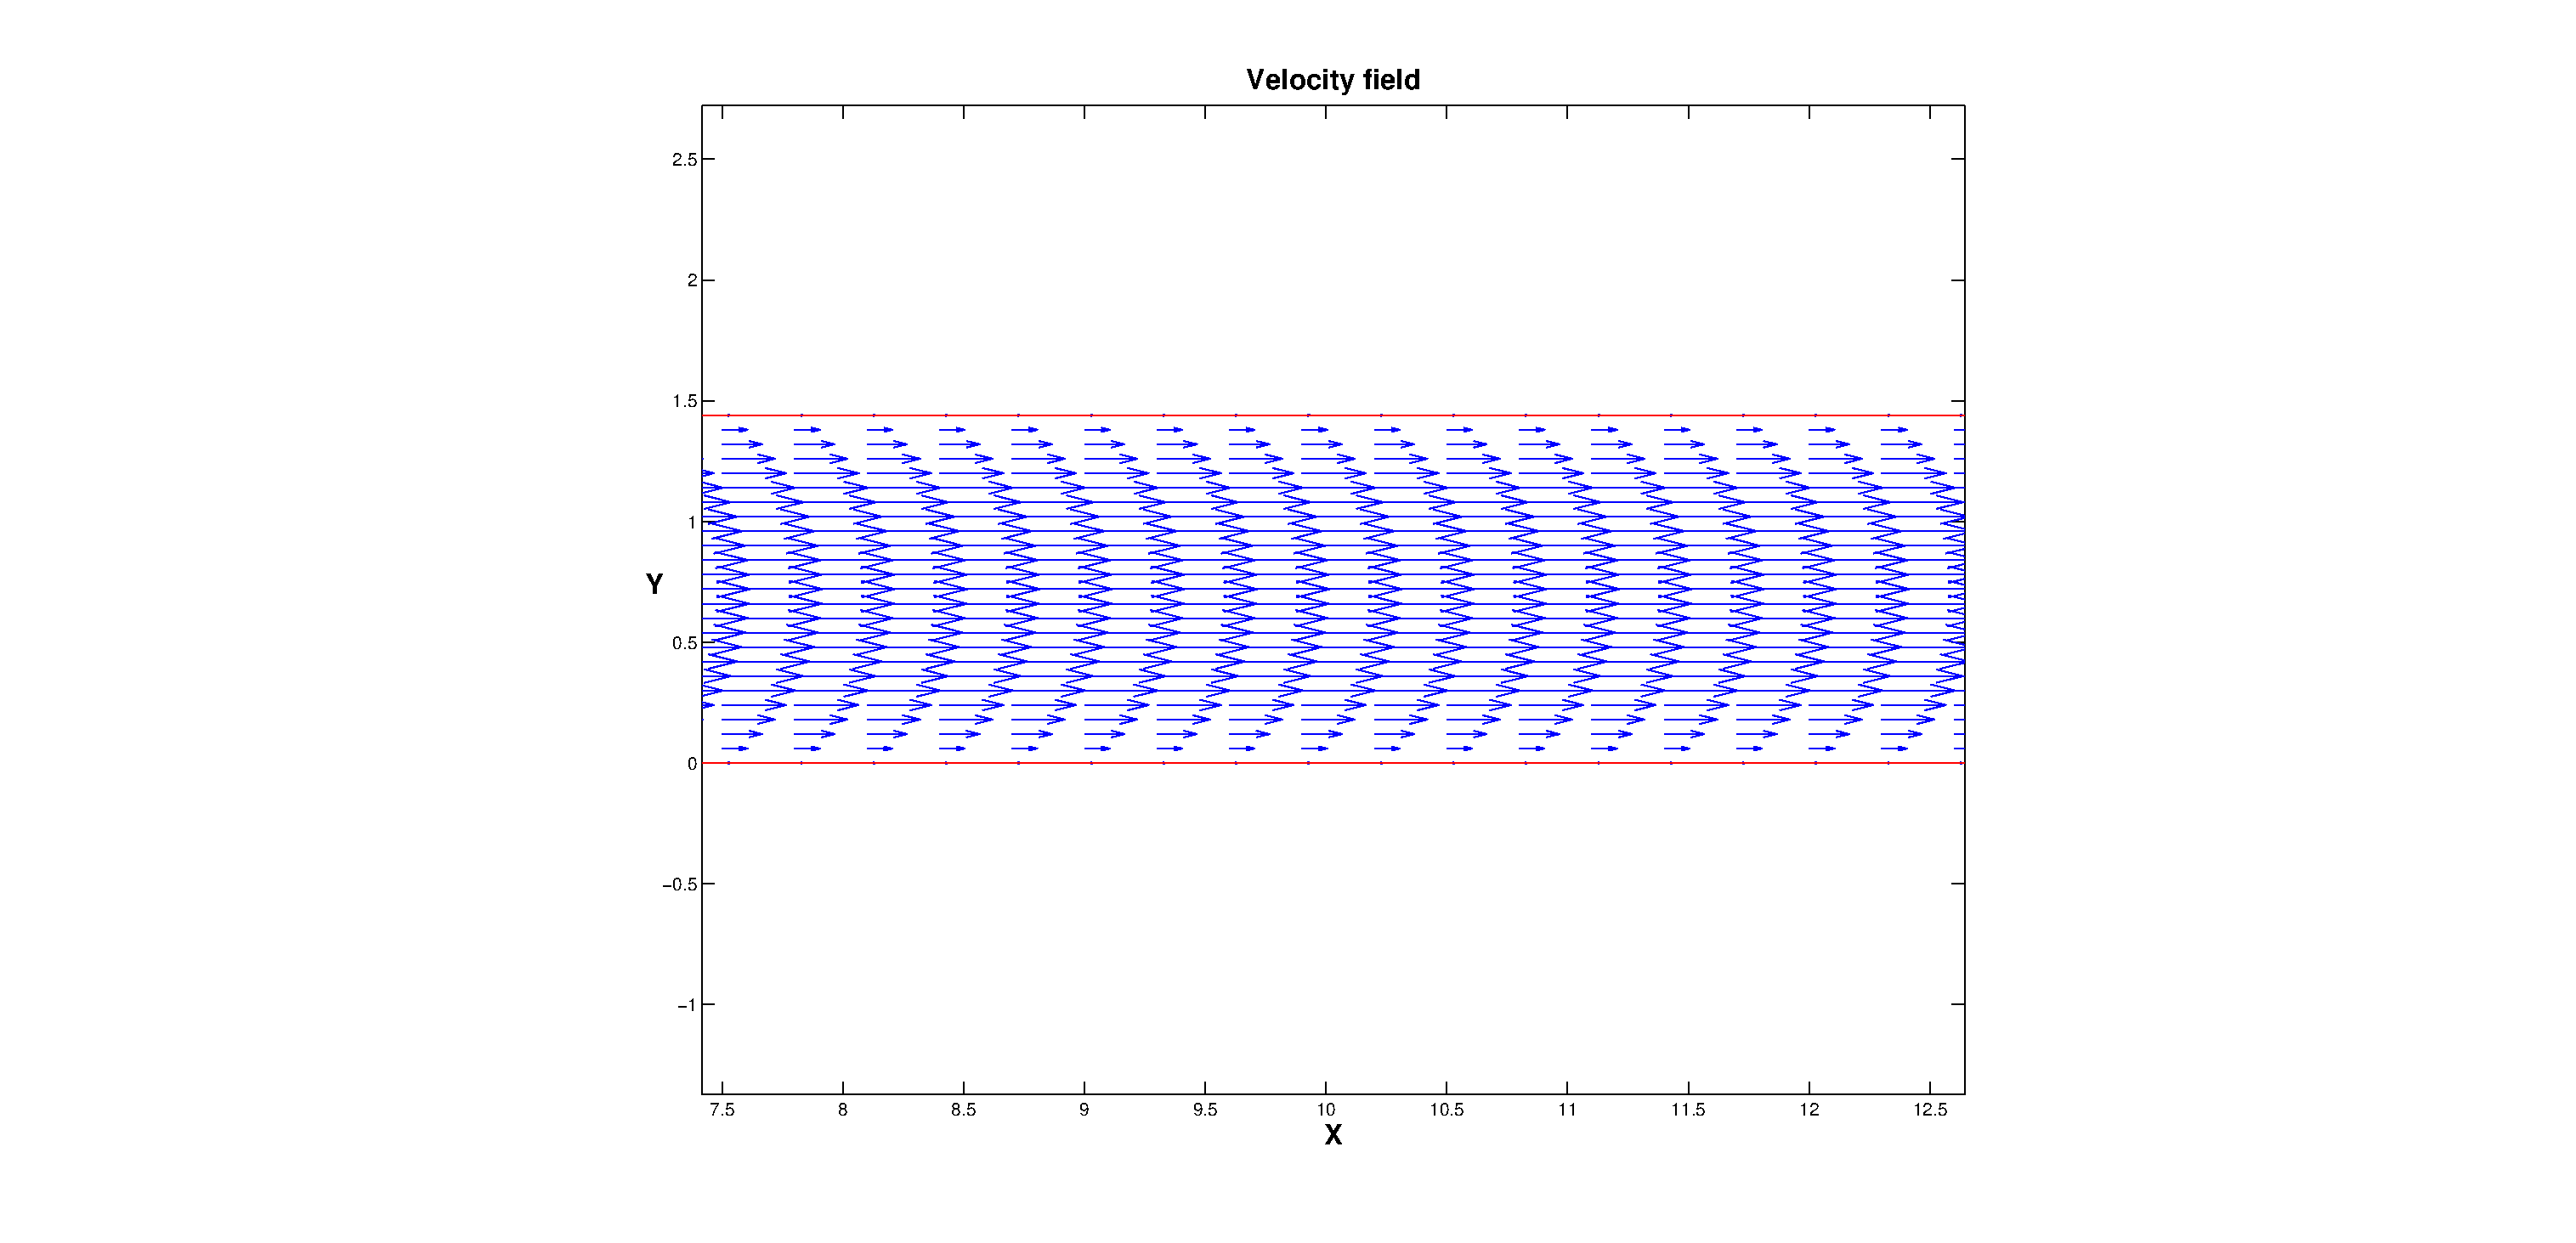
\includegraphics[scale=.3]{pplate500_velocityfield.eps}
\end{center}
\caption{Flow Between Two Parallel Plates at Re = 500}
\end{figure}

The velocity profile of a fluid flow driven by an inflow between two parallel plates is given in figure(\ref{fbtpp500}) for $Re = 500$ . We employ the same inflow velocity as before in all our simulations. In the case where $Re = 500,000$ the effect of viscosity is pronounced in a small layer close to the boundary. This small region is known as the boundary layer \cite{fmln}. Outside of this region, the flow is almost uniform.

\section{Lid-Driven Cavity Flow}

We investigate flow in a lid-driven cavity. We use the no-slip condition on the four boundaries with the lid having a constant velocity of $(1,0)$. The computational domain has dimension $1\times1$ subdivided into equally spaced subintervals in both the $x$ and $y$ directions. The Reynolds number used for this flow is $100$.  

\begin{figure}
\label{ldc1}
\begin{center}
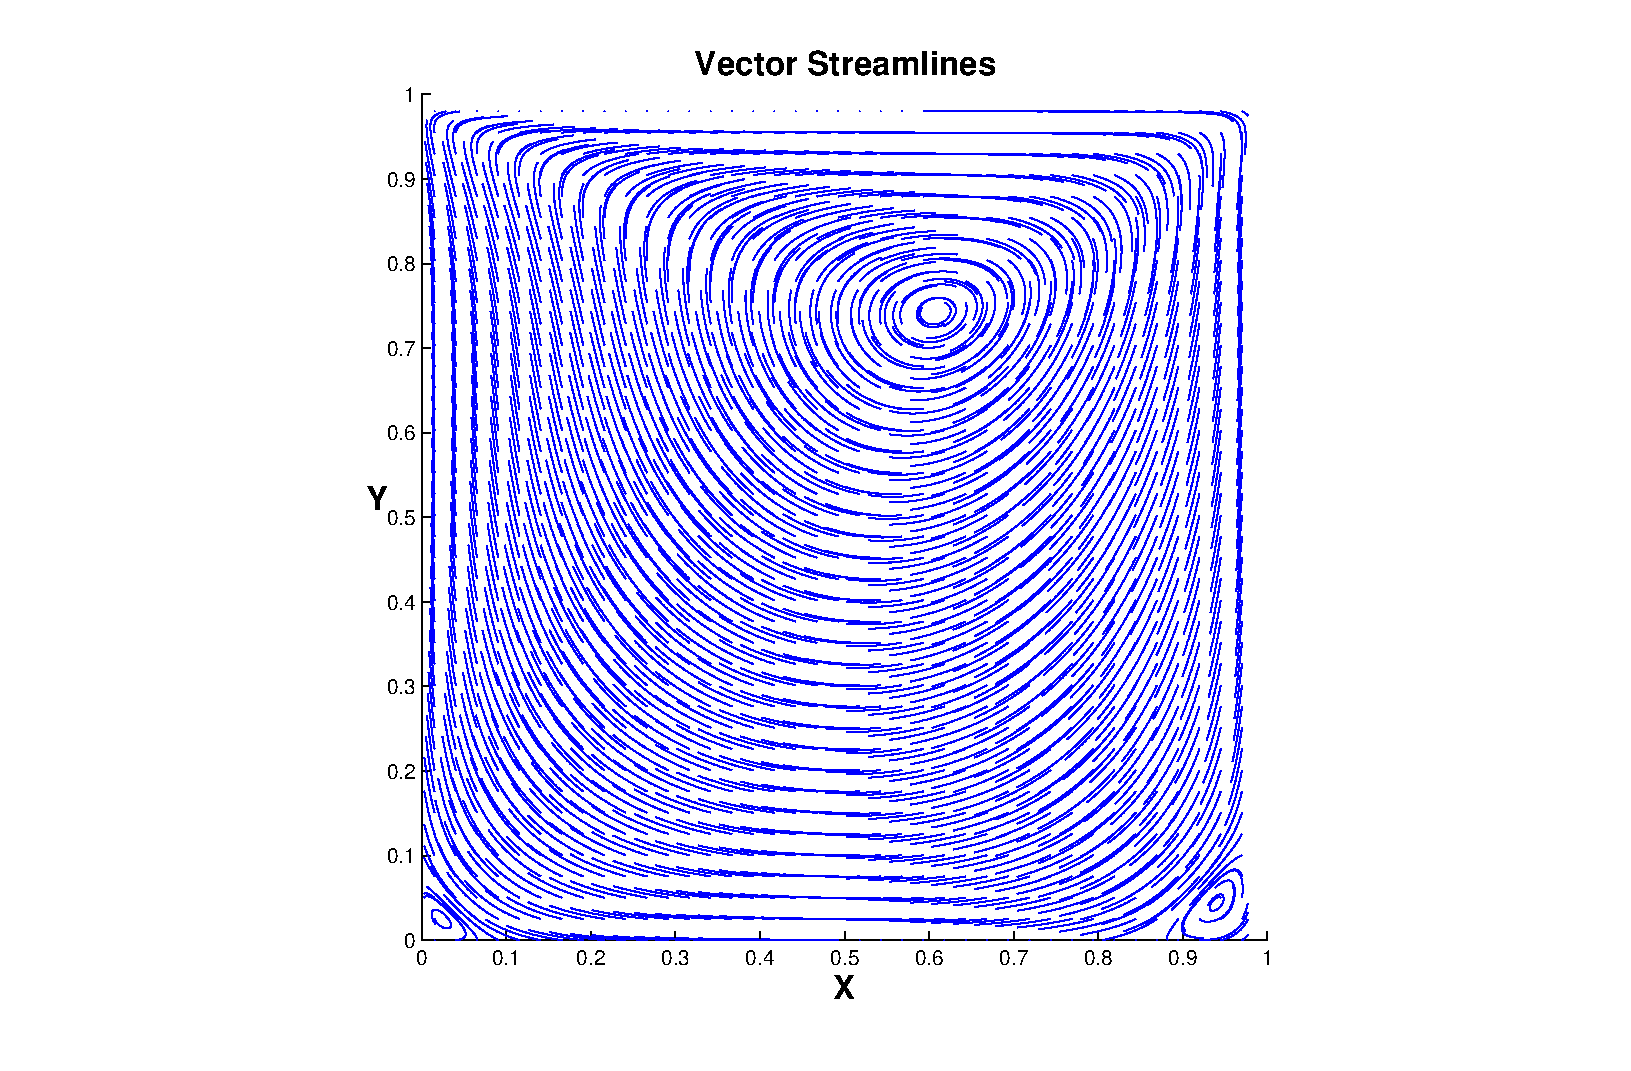
\includegraphics[scale=.5]{dcavity.eps}
\end{center}
\caption{Flow in a Lid-Driven Cavity}
\end{figure}

When the parameters are chosen as above, these regions of recirculation known as eddies are formed in the two lower corners of the cavity. 

\begin{figure}
\label{ldc2}
\begin{center}
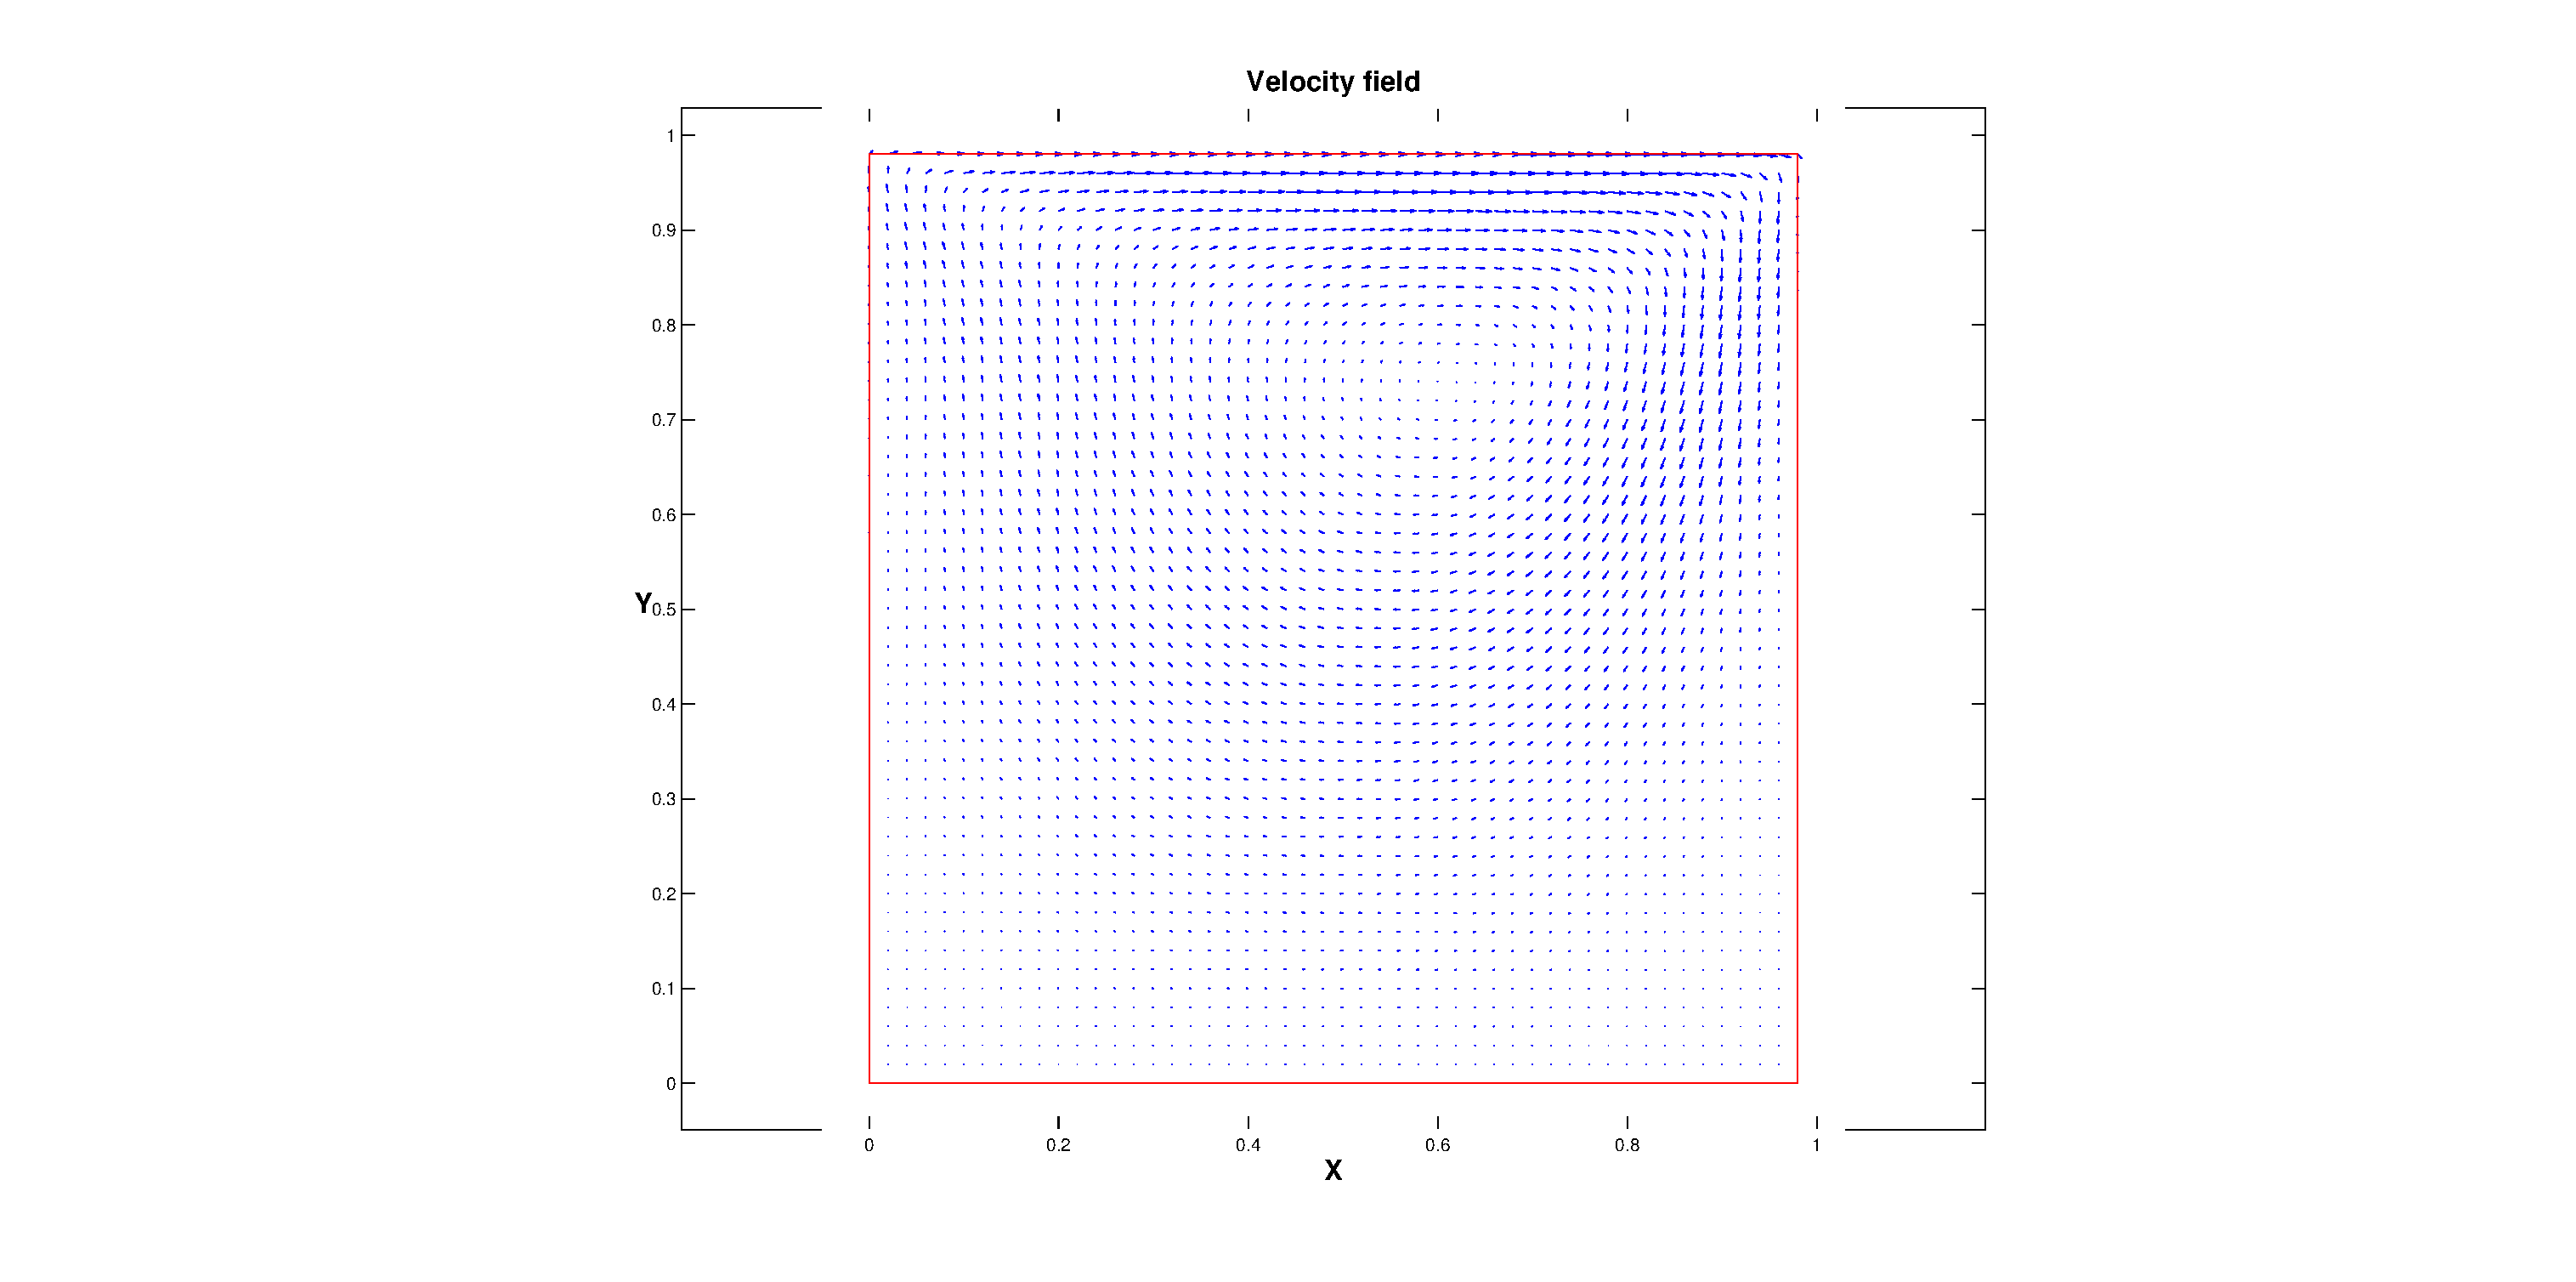
\includegraphics[scale = .3]{dcavity_velocityfield.eps}
\end{center}
\caption{Flow in a Lid-Driven Cavity}
\end{figure}

\section{Flow Over a Backward Facing Step}

We investigate flow over a backward facing step. We take the no-slip condition on the north and south boundaries and the inflow/outflow condition on the east and west boundaries. The initial inflow velocity in the horizontal direction is set to $1$ and the vertical component is set to $0$. The dimension of the domain is $30\times1.5$ in which the $x$-direction is subdivided into $100$ equally spaced subintervals and the $y$-direction is subdivided into $25$ equally spaced subintervals.The Reynolds number used for this flow is $500$. It can be seen that there is a recirculation region behind the step as one expects. 

\begin{figure}
\begin{center}
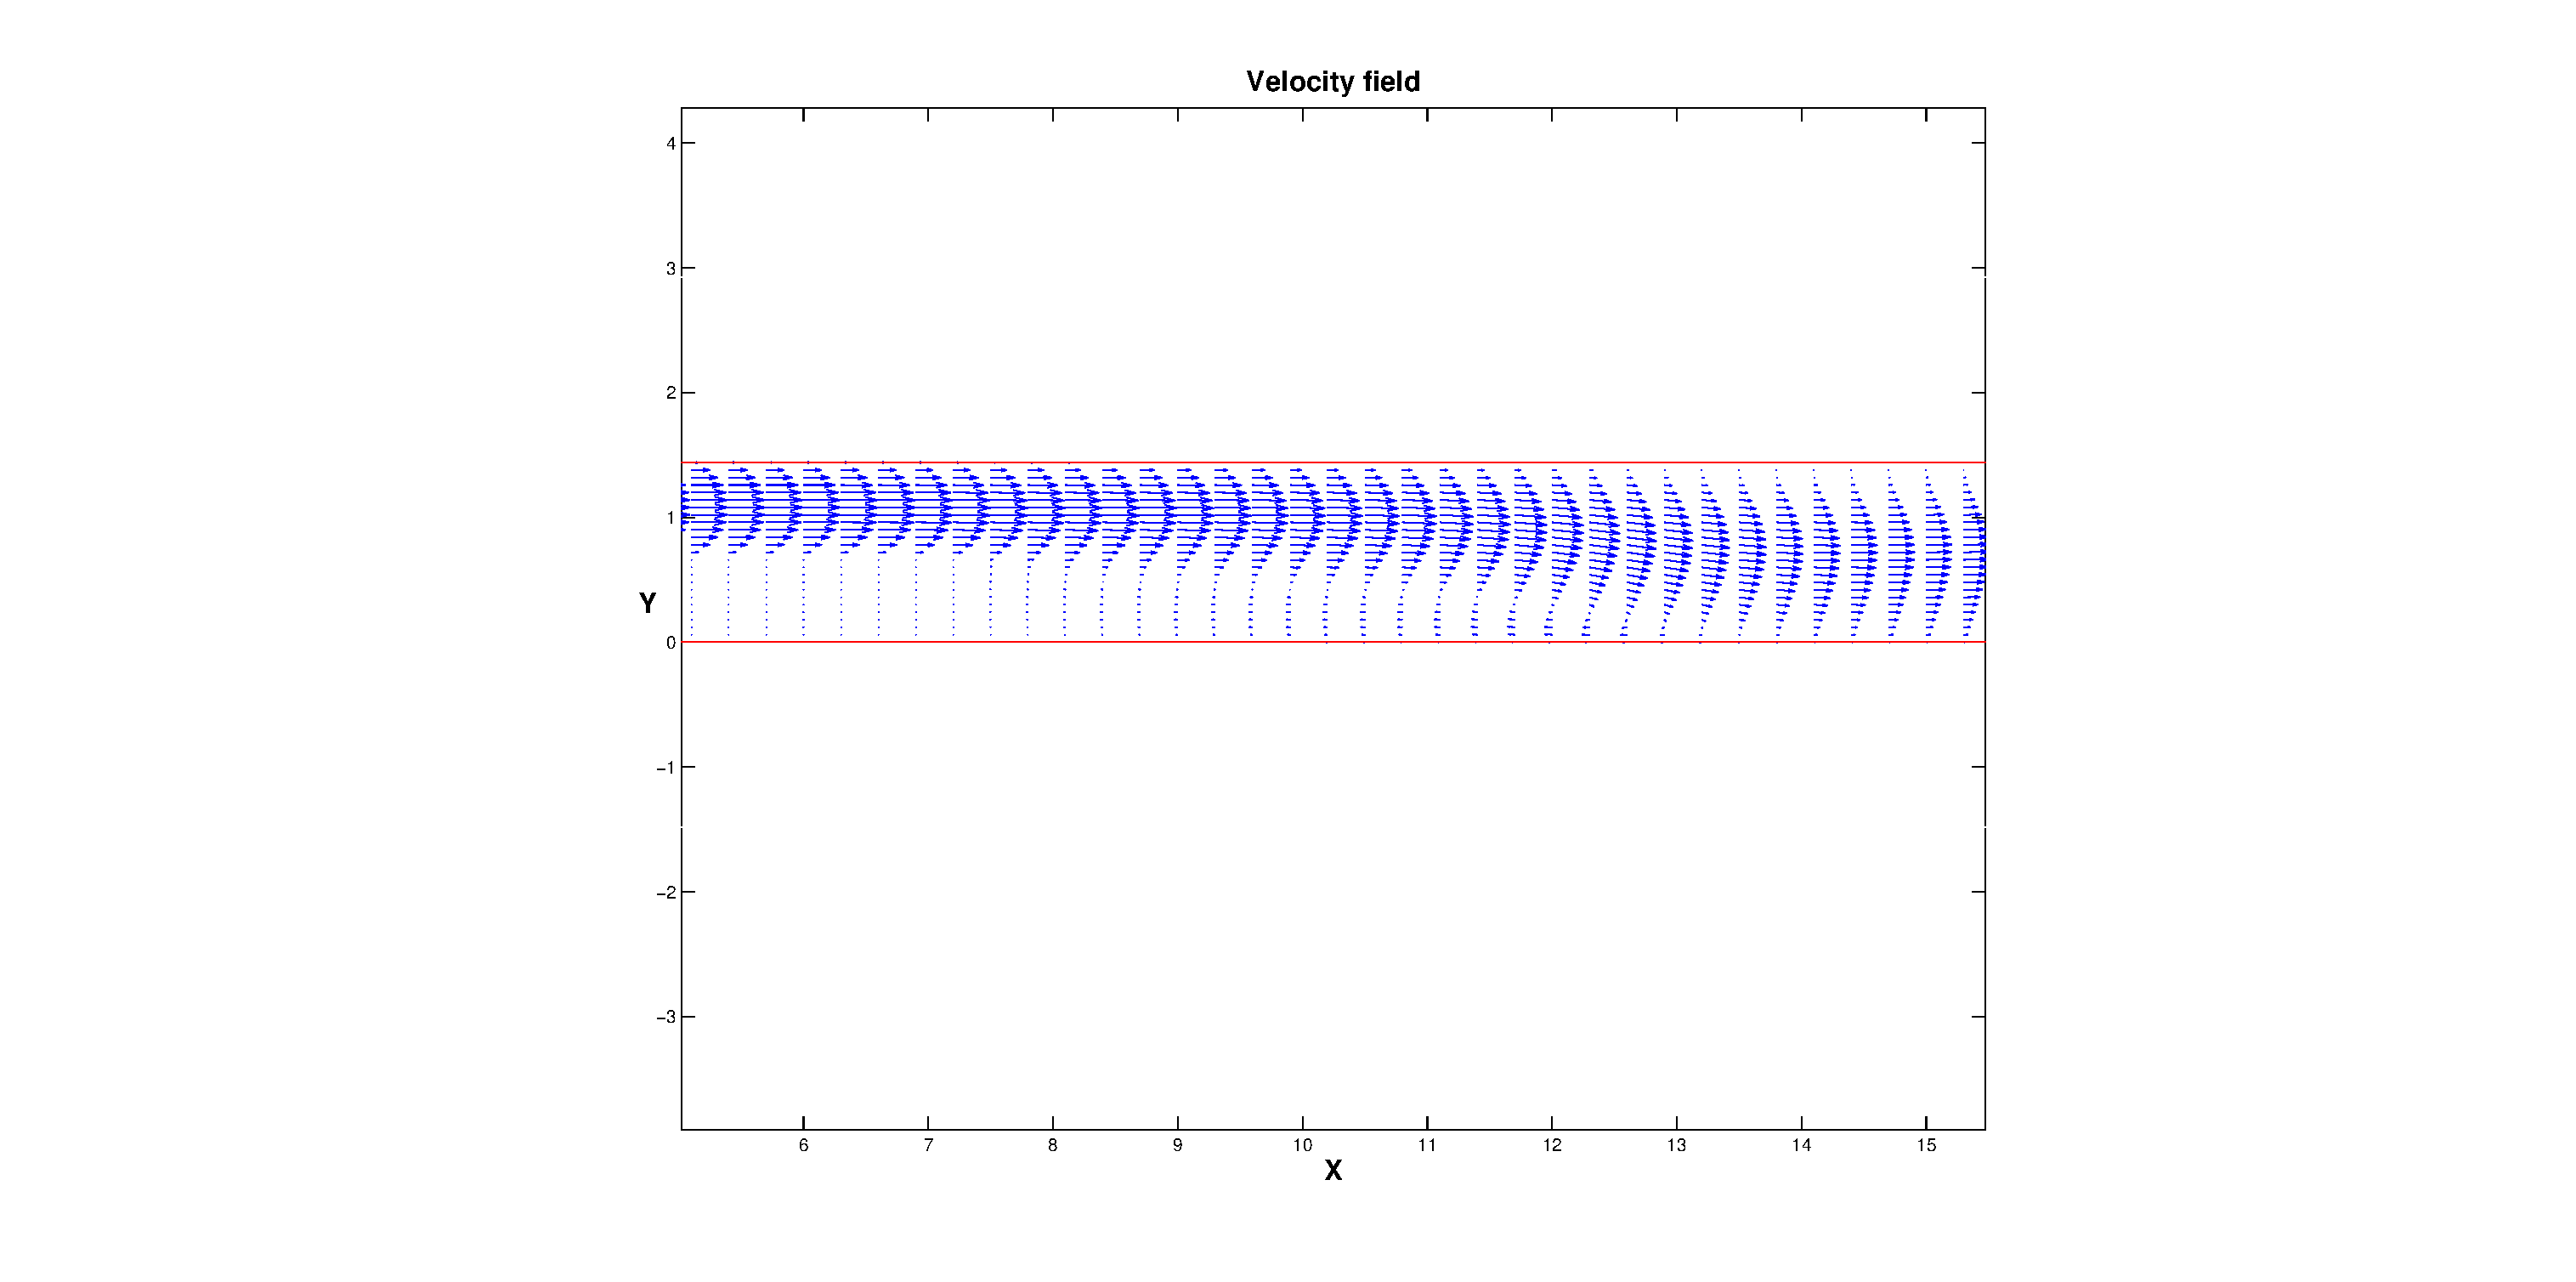
\includegraphics[scale=.3]{backstep_velocityfield.eps}
\end{center}
\caption{Flow Past a Backward Facing Step.}
\label{bwfs1}
\end{figure}

\begin{figure}
\begin{center}
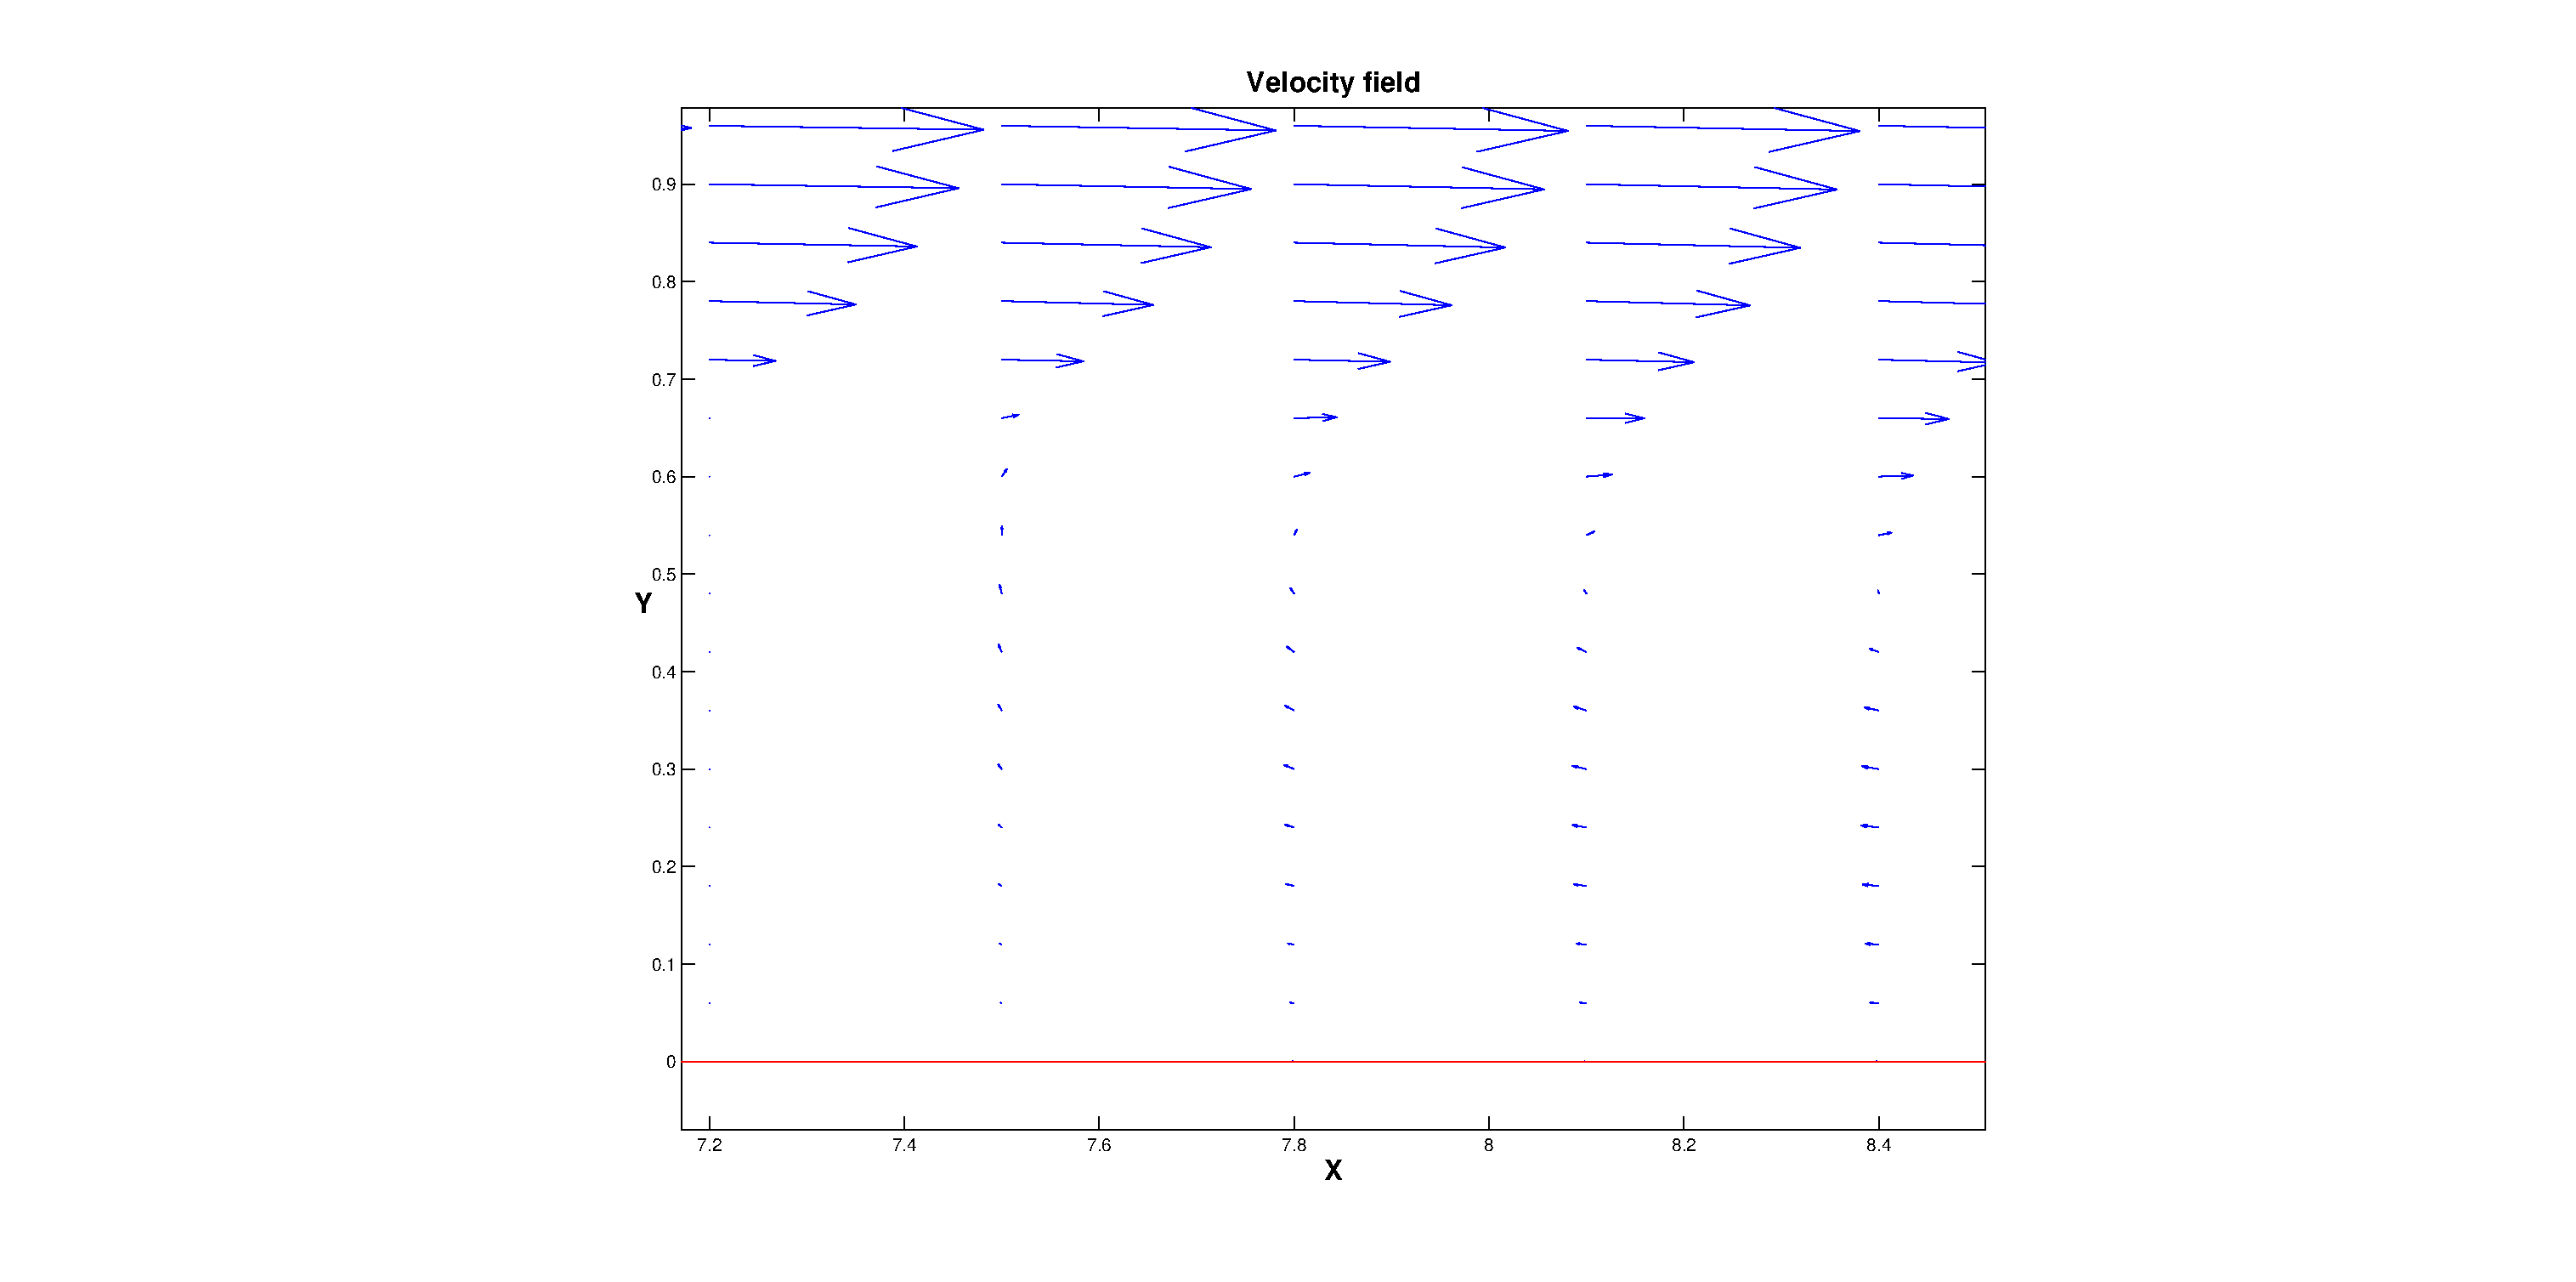
\includegraphics[scale=.3]{backstep_velocityfield1.eps}
\end{center}
\caption{Flow Past a Backward Facing Step.}
\label{bwfs2}
\end{figure}

\section{Conclusion}

In this chapter, flow between two parallel plates, flow in a lid-driven cavity, and flow over a backward facing step are investigated. The effects of different Reynold's numbers is also presented. We conclude by summarizing what has been done. 
%\end{document}